% !TeX program = xelatex
% !TeX encoding = UTF-8
\documentclass{MathorCupmodeling}
\usepackage{mwe,color,float}
\usepackage[linesnumbered,ruled]{algorithm2e}
\everymath{\displaystyle}

\extrafloats{100}
\bianhao{MC2305806}
\tihao{题号}
\timu{\textbf{题目}}
\keyword{关键词两个之间分号隔开}
\begin{document}
	\begin{abstract}
		这里是摘要部分
	\end{abstract}

	\pagestyle{empty}
	\tableofcontents
	\newpage
	\pagestyle{fancy}

	\setcounter{page}{1}
	\section{问题的提出}
	\subsection{问题背景}
	问题背景
	\subsection{问题要求}
	\begin{itemize}
		\item \textbf{问题一}:
		\item \textbf{问题二}:
		\item \textbf{问题三}:
		\item ……
	\end{itemize}

	\section{问题的分析}
	\subsection{问题的整体分析}

	\textbf{从分析目的看},分析目的Ctrl+Alt+B

	\textbf{从数据来源、特征看},
	
	\textbf{从模型的选择看},

	\textbf{从软件的选择看},
	
	\subsection{问题一的分析}
	问题一的分析xxx
	\subsection{问题二的分析}

	\section{模型的假设}
	\begin{itemize}
		\item \textbf{假设一}:
		\item \textbf{假设二}:
		\item \textbf{假设三}:
		\item \textbf{假设四}:
		\item ……
	\end{itemize}
	\section{符号说明}
	\begin{center}
		\begin{tabularx}{0.7\textwidth}{c@{\hspace{1pc}}|@{\hspace{2pc}}X}
			\Xhline{0.08em}
			符号 & \multicolumn{1}{c}{符号说明}\\
			\Xhline{0.05em}
			$\mu$ & 样本平均数 \\
			$\alpha$ & 系数 \\
			$\beta$ & \\
			$\omega$ & \\
			$\sigma$ & 标准差 \\
			\Xhline{0.08em}
		\end{tabularx}
	\end{center}

	\section{模型的建立与求解}
	\subsection{问题一模型的建立}
	这里是图片的演示,见\textcolor{blue}{\cref{fig:picturename1}}。
	\begin{figure}[H]
		\centerline{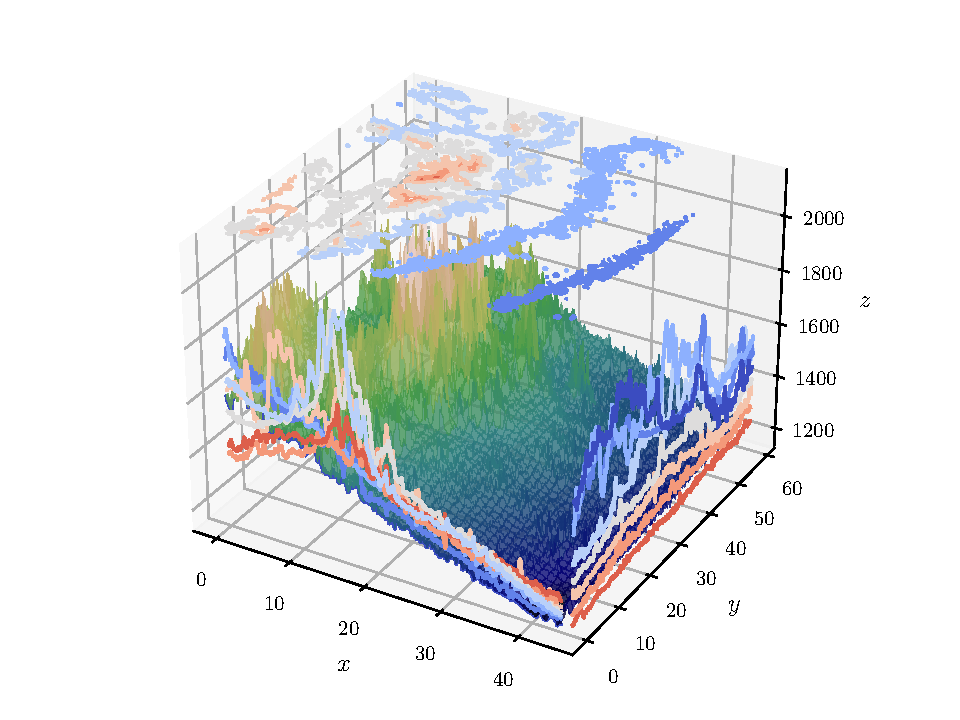
\includegraphics[scale=0.8]{三维网格图.pdf}}
		\caption{这里是图片的标题}\label{fig:picturename1}
	\end{figure}
	这里是第二张图片的延时,见\textcolor{blue}{\cref{fig:picturename2}}。
	\begin{figure}[H]
		\centerline{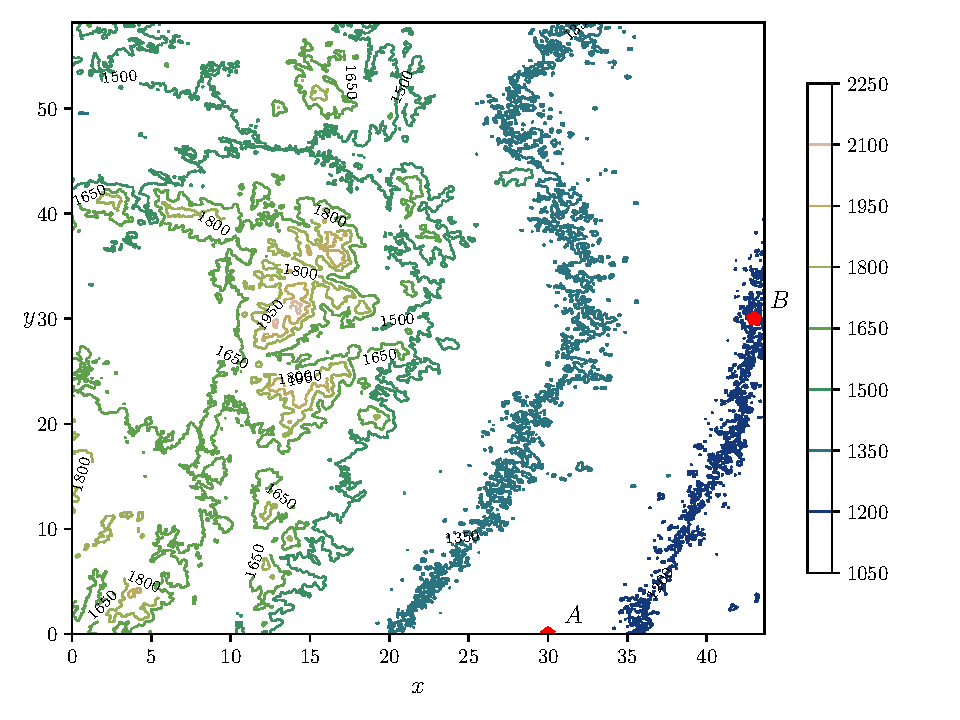
\includegraphics[scale=0.8]{等高线图.pdf}}
		\caption{这里是图片的标题}\label{fig:picturename2}
	\end{figure}
	假如这段话是引用了话,要有注释喔!\textcolor{blue}{\cite{p1}}
	这里我们还可以做个脚注。\textcolor{blue}{\footnote{脚注的内容}}

	这里我们做一个表格,三线表喔!见\textcolor{blue}{\cref{tab:tablename1}}。
	\begin{table}[htbp]
	\centering
	\caption{标题在这里!~}
	\setlength{\aboverulesep}{0pt}
	\setlength{\belowrulesep}{0pt}
	\scalebox{0.88}{
	  \begin{tabular}{ccc}
	  \toprule
	  A     & B     & C \\
	  \midrule
	  1     & 12    & hello \\
	  2     & E     & 汉字 \\
	  3     & apple & pear \\
	  \bottomrule
	  \end{tabular}}
	\label{tab:tablename1}
  	\end{table}
	结果见\textcolor{blue}{\cref{tab:firsttable}}。
	\begin{table}[H]
	\centering
	\caption{表格名称}
	  \begin{tabular}{ccc}
	  \toprule
	  A     & B     & C \\
	  \midrule
	  1     & 2     & 3 \\
	  一     & 二     & 三 \\
	  1     & 2.98  & 3.97 \\
	  \bottomrule
	  \end{tabular}
	\label{tab:firsttable}
 	\end{table}
  % Table generated by Excel2LaTeX from sheet 'Sheet1'
\begin{table}[htbp]
	\centering
	\caption{Add caption}
	\setlength{\aboverulesep}{0pt}
	\setlength{\belowrulesep}{0pt}
	\scalebox{0.5}{
	  \begin{tabular}{c|cc}
	  \toprule
	  A     & B     & C \\
	  \midrule
	  1     & 2     & 3 \\
	  一     & 二     & 三 \\
	  1     & 2.98  & 3.97 \\
	  \bottomrule
	  \end{tabular}}
	\label{tab:addlabel}
  \end{table}
  
这个公式$\frac{x^2}{5}+\frac{y^2}{4}=1$是行内公式
下面的公式为行间公式:
$$
E=\int \frac{\mathrm{d}q}{4\pi \varepsilon_0 r^2}
$$
$$
\sum_{i = 1}^\infty  {\frac{5}{i}}
$$
行内求和$\sum\limits_{i = 1}^\infty  {\frac{5}{i}}$
第二种行间公式如下\textcolor{blue}{\cref{eqone}}
\begin{equation}\label{eqone}
E=\int \frac{\mathrm{d}q}{4\pi \varepsilon_0 r^2}
\end{equation}
	\section{模型的评价与推广}
	\begin{figure}[H]
		\centering{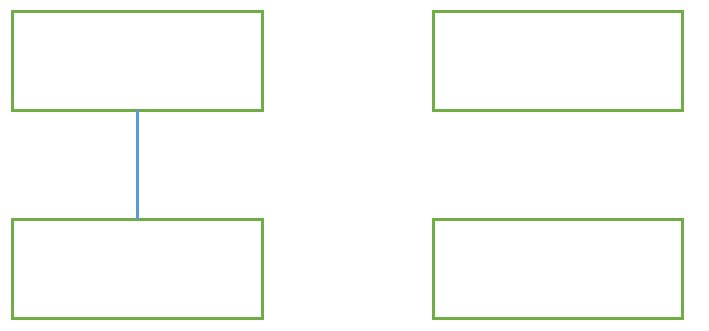
\includegraphics[scale=0.8]{文字文稿1.pdf}}
		\caption{这里是图片的标题}\label{fig:picturename3}
	\end{figure}
	\subsection{模型的评价}
	\begin{itemize}
		\item \textbf{模型的优点}:
			\begin{enumerate}
				\item ……
				\item ……
			\end{enumerate}
		\item \textbf{模型的缺点}:
			\begin{enumerate}
				\item ……
				\item ……
				\item ……
			\end{enumerate}
		\item \textbf{模型的改进}:
			\begin{enumerate}
				\item ……
				\item ……
				\item ……
			\end{enumerate}
	\end{itemize}
	\subsection{模型的推广}

	\newpage
	\phantomsection
	\addcontentsline{toc}{section}{\textbf{参考文献}}
	\begin{thebibliography}{99}
	\bibitem{p1}张学工.关于统计学习理论与支持向量机[J].自动化学报,2000(01):36-46.DOI:10.16383/j.aas.2000.01.005.
	
	\end{thebibliography}

	\newpage

	\phantomsection
	\addcontentsline{toc}{section}{\textbf{附\hspace{2pc}录}}

	% \appendix
	% \ctexset{section={format={\zihao{-4}\heiti\raggedright}}}
	\begin{center}
		\heiti\zihao{4} 附\hspace{2pc}录
	\end{center}

% \phantomsection
% \addcontentsline{toc}{subsection}{[A]图示}
	% \section*{[A]图示}
	\noindent{\heiti [A]图示}

\newpage
% \phantomsection
% \addcontentsline{toc}{subsection}{[B]支撑文件列表}
	% \section*{[B]支撑文件列表}
	\noindent{\heiti [B]支撑文件列表}
	~\\

	支撑文件列表如下(列表中不包含原始数据集):

\newpage
% \phantomsection
% \addcontentsline{toc}{subsection}{[C]使用的软件、环境}
	% \section*{[C]使用的软件、环境}
	\noindent{\heiti [C]使用的软件、环境}
	~\\

	为解决该问题,我们所使用的主要软件有:
	
	Python环境下所用使用到的库及其版本如下:

\newpage
% \phantomsection
% \addcontentsline{toc}{subsection}{[D]问题解决源程序}
	% \section*{[D]问题解决源程序}
\noindent{\heiti [D]问题解决源程序}

% \phantomsection
% \addcontentsline{toc}{subsubsection}{D.1}
\textbf{D.1 }
\begin{python}
import numpy as np
\end{python}
\newpage
% \phantomsection
% \addcontentsline{toc}{subsubsection}{D.2}
\textbf{D.2 }

\newpage
% \phantomsection
% \addcontentsline{toc}{subsubsection}{D.3}
\textbf{D.3 }

\newpage
% \phantomsection
% \addcontentsline{toc}{subsubsection}{D.4}
\textbf{D.4 }

\end{document}